%% Author: Leighton Pritchard
%% Copyright: James Hutton Institute
%% 2014-11-21: Slides for teaching at University of Strathclyde, 21st November 2014
%% This presentation was an invited guest lecture on microbial genomics and bioinformatics
%% for the BM405 course.

%% UNCOMMENT FOR SLIDES
\documentclass[table]{beamer}
\mode<presentation>

%% UNCOMMENT FOR HANDOUTS
%\documentclass[handout]{beamer}
\usepackage{handoutWithNotes}
\pgfpagesuselayout{4 on 1 with notes}[a4paper,border shrink=5mm]

%% GENERIC STYLE SETTINGS BELOW
\usetheme{default}
\usepackage{listings}
\usepackage{multirow}
\usepackage{xcolor}
\usepackage{hyperref}

\usebackgroundtemplate{

\includegraphics[width=\paperwidth,height=\paperheight]{images/hutton_background}
}
%% PRESENTATION CONFIGURATION PARAMETERS %%%%%%%%%%%%%%%%%%%%%%%%%%%%%%%%%%%%%%%
%\titlebackgroundfile{images/hutton_title}
%\framebackgroundfile{images/hutton_background}
\definecolor{hutton_green}{HTML}{78A22F}
\definecolor{hutton_purple}{HTML}{872175}
\definecolor{hutton_blue}{HTML}{569BBE}
\usefonttheme{structurebold}
\setbeamercolor{alerted text}{fg=orange}
\setbeamercolor{background canvas}{bg=white}
\setbeamercolor{block title}{bg=hutton_purple}
\setbeamercolor{frametitle}{fg=hutton_purple}
\setbeamercolor{title}{fg=black}
\setbeamercolor{titlelike}{fg=hutton_green}
\setbeamercolor{author}{fg=hutton_purple}
\setbeamercolor{author in head/foot}{fg=white}
\setbeamercolor{title in head/foot}{fg=white}
\setbeamercolor{section in head/foot}{fg=hutton_purple}
\setbeamercolor{normal text}{fg=black}
\setbeamercolor{frametitle}{fg=hutton_purple}
\setbeamerfont{block title}{size={}}
\setbeamerfont{author}{size=\footnotesize}
\setbeamerfont{institute}{size=\tiny}
\setbeamerfont{date}{size=\footnotesize}
\setbeamercolor{section in toc shaded}{fg=hutton_purple}
\setbeamercolor{section in toc}{fg=hutton_purple}
\setbeamercolor{subsection in toc shaded}{fg=hutton_purple}
\setbeamercolor{subsection in toc}{fg=hutton_purple}
\setbeamertemplate{itemize item}[circle]
\setbeamertemplate{itemize subitem}[circle]
\setbeamertemplate{itemize subsubitem}[circle]
\setbeamertemplate{itemize subsubsubitem}[circle]
\setbeamercolor{itemize item}{fg=hutton_purple}
\setbeamercolor{itemize subitem}{fg=hutton_purple}
\setbeamercolor{itemize subsubitem}{fg=hutton_purple}
\setbeamercolor{itemize subsubsubitem}{fg=hutton_purple}
\setbeamercolor{enumerate item}{fg=hutton_purple}
\setbeamercolor{enumerate subitem}{fg=hutton_purple}
\setbeamercolor{enumerate subsubitem}{fg=hutton_purple}
\setbeamercolor{enumerate subsubsubitem}{fg=hutton_purple}
\setbeamercolor{alerted text}{fg=hutton_green}
\setbeamerfont{alerted text}{series=\bfseries}
% This command makes sure that acrobat reader doesn't change the colours of the slide
% when there are figures with transparencies.
\pdfpageattr {/Group << /S /Transparency /I true /CS /DeviceRGB>>}

%Disables discrete bottom navigation bar
%\beamertemplatenavigationsymbolsempty

% Modify the slide titles to avoid the corner images,
\setbeamertemplate{frametitle}
{
\vspace{0.05\textheight}
\noindent\quad\begin{minipage}[t][0.12\textheight][t]{0.85\textwidth}
\insertframetitle\par
\end{minipage}
}

% Modify title page to avoid the big logo on right
\setbeamertemplate{title page}{
    \begin{picture}(0,0)
            %This ends up on top of the default background image, rather than replacing it:
            \put(-30,-165){%
                
\includegraphics[width=\paperwidth,height=\paperheight]{images/hutton_title}
            }
            \put(0,-75){%
                \begin{minipage}[b][0.4\textheight][t]{0.75\textwidth}
                    \usebeamerfont{title}\usebeamercolor[fg]{title}{\inserttitle\par}
                    \usebeamerfont{subtitle}\usebeamercolor[fg]{subtitle}{\insertsubtitle\par}
                \end{minipage}
            }
            \put(0,-125){%
                \begin{minipage}[b][0.1\textheight][t]{\textwidth}
                    \usebeamerfont{author}\usebeamercolor[fg]{author}{\insertauthor\par}
                    \usebeamerfont{institute}\usebeamercolor[fg]{institute}{\insertinstitute\par}
                \end{minipage}
            }
    \end{picture}
}

%%%%%%%%%%%%%%%%%%%%%%%%%%%%%%%%%%%%%%%%%%%%%%%%%%%%%%%%%%%%%%%%%%%%%%%%%%%%%%%%

% LISTINGS SETTING
% Settings for code listings in lstlistings

\definecolor{hutton_lightgreen}{HTML}{C8F27F}

\lstset{ %
  backgroundcolor=\color{hutton_lightgreen},   % choose the background color; you must add \usepackage{color} or \usepackage{xcolor}
  basicstyle=\tiny\ttfamily,        % the size of the fonts that are used for the code
  breakatwhitespace=false,         % sets if automatic breaks should only happen at whitespace
  breaklines=true,                 % sets automatic line breaking
  captionpos=b,                    % sets the caption-position to bottom
  commentstyle=\color{red},    % comment style
  deletekeywords={...},            % if you want to delete keywords from the given language
  escapeinside={\%*}{*)},          % if you want to add LaTeX within your code
  extendedchars=true,              % lets you use non-ASCII characters; for 8-bits encodings only, does not work with UTF-8
  frame=single,                    % adds a frame around the code
  keepspaces=true,                 % keeps spaces in text, useful for keeping indentation of code (possibly needs columns=flexible)
  keywordstyle=\color{blue},       % keyword style
%  language=Octave,                 % the language of the code
  morekeywords={*,...},            % if you want to add more keywords to the set
  numbers=left,                    % where to put the line-numbers; possible values are (none, left, right)
  numbersep=5pt,                   % how far the line-numbers are from the code
  numberstyle=\tiny\color{gray}, % the style that is used for the line-numbers
  rulecolor=\color{black},         % if not set, the frame-color may be changed on line-breaks within not-black text (e.g. comments (green here))
  showspaces=false,                % show spaces everywhere adding particular underscores; it overrides 'showstringspaces'
  showstringspaces=false,          % underline spaces within strings only
  showtabs=false,                  % show tabs within strings adding particular underscores
  stepnumber=1,                    % the step between two line-numbers. If it's 1, each line will be numbered
  stringstyle=\color{violet},     % string literal style
  tabsize=4,                       % sets default tabsize to 2 spaces
  title=\lstname                   % show the filename of files included with \lstinputlisting; also try caption instead of title
}


%%%
% TITLE PREAMBLE
\title[Microbial Genomics and Bioinformatics: 2.Assembly] % (optional, only for long titles)
{Microbial Genomics and \\ Bioinformatics \\
BM405 \\
2.Assembly}
%\subtitle{}
\author[Pritchard] % (optional, for multiple authors)
{Leighton~Pritchard$^{1,2,3}$}
\institute[The James Hutton Institute] % (optional)
{
  $^{1}$Information and Computational Sciences,\\
  $^{2}$Centre for Human and Animal Pathogens in the Environment,\\
  $^{3}$Dundee Effector Consortium,\\
  The James Hutton Institute, Invergowrie, Dundee, Scotland, DD2 5DA
}
\date[21st November 2014] % (optional)
{21st November 2014}
\subject{Bioinformatics, Genomics, Bacteria, Sequencing, Microbiology, Microbes}

%%%
% TOC
% Show table of contents, with current section highlighted,
% at the start of each section

%\AtBeginSection[]
%{
%  \begin{frame}
%    \frametitle{Table of Contents}
%    \tableofcontents[currentsection] %,hideallsubsections]
%  \end{frame}
%}

\AtBeginSubsection[]
{
  \begin{frame}
    \frametitle{Table of Contents}
    \tableofcontents[currentsection,currentsubsection] %,hideallsubsections]
  \end{frame}
}

%%%
% START DOCUMENT
\begin{document}

\frame[plain]{\titlepage}

%% use.tex
%% Author: Leighton Pritchard
%% Copyright: James Hutton Institute
%% These slides describe the acceptable use policy for these slides and
%% materials

%
\begin{frame}
  \frametitle{Acceptable Use Policy}
  Recording of this talk, taking photos, discussing the content using \\
  email, Twitter, blogs, etc. is permitted (and encouraged), \\
  providing distraction to others is minimised. \\[0.5cm]
  These slides will be made available on SlideShare. \\[0.5cm]
  These slides, and supporting material, are available at \href{https://github.com/widdowquinn/Teaching-2014-11-21-Strathclyde}{https://github.com/widdowquinn/Teaching-2014-11-21-Strathclyde}
\end{frame}

%%%
% SECTION: Sequence Data Formats
\section{Sequence Data Formats}
%% read_data_formats.tex
%% Author: Leighton Pritchard
%% Copyright: James Hutton Institute
%% These slides briefly introduce the ways in which sequence 
%% data tends to arrive at the bioinformatician

% The two main current sequence read data formats
\begin{frame}
  \frametitle{What do you get from sequencing\footnote{\tiny{Miyamoto \textit{et al}. (2014) \textit{BMC Genomics} \textbf{15}:699 \href{http://dx.doi.org/10.1186/1471-2164-15-699}{doi:10.1186/1471-2164-15-699}}}}
  Sequence reads. Lots of them. \\
  Size/number depend on technology used.
    \begin{center}
      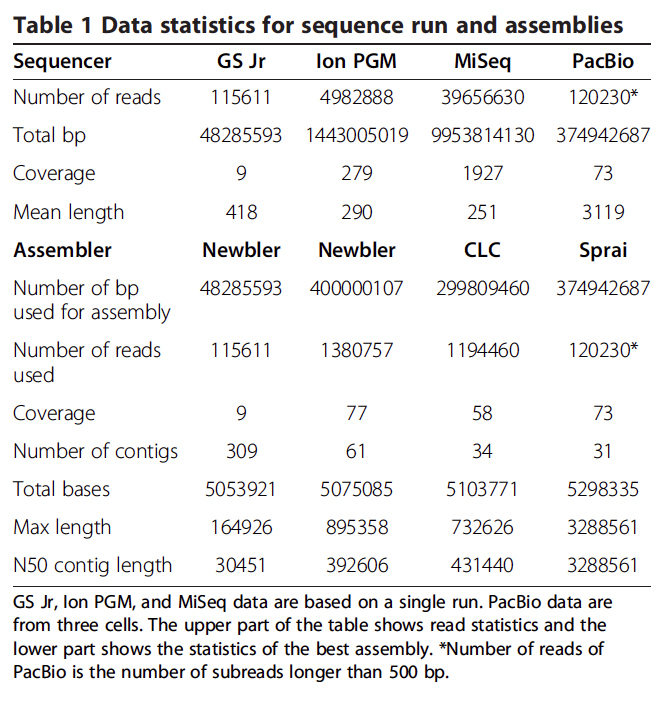
\includegraphics[height=0.7\textheight]{images/miyamoto_table}
    \end{center}   
\end{frame}

% The two main current sequence read data formats
\begin{frame}
  \frametitle{Sequence Read Data Formats}
  Two common read data sequence formats:
  \begin{itemize}
    \item \textbf{FASTQ}: Related to FASTA, a \textit{de facto} standard for sequence reads
    \item \textbf{SAM/BAM}: Sequence alignment/mapping format, two flavours - uncompressed and compressed
    \item \textbf{CRAM}: Reference-based sequence compression
  \end{itemize}
  You might also receive assembled genomes directly from a sequencing partner
\end{frame}

% SUBSECTION: FASTQ
% A very brief summary of the FASTQ format
\subsection{FASTQ}

% FASTQ data format
\begin{frame}[fragile]
  \frametitle{FASTQ\footnote{\tiny{\href{http://dx.doi.org/10.1093/nar/gkp1137}{Cock \textit{et al}. (2009) \textit{Bioinformatics} \textbf{38}:1767-1771 doi:10.1093/nar/gkp1137}}}}
\begin{verbatim}
@HISEQ2500-09:168:HA424ADXX:2:1101:1404:2061 1:N:0:ATCTCTCTCACCAACT
CGGTCTTGGGATAGATGGGTTGCAGGTTGCGGTAAAGCTCGGACTCCAGAGCGTCCAGGGTAGACTGGCTAATCTTCTGCTCTTTATCGATCATTATTTC
+
@@CBDDFFHHDFDHEGHIICGIFHHIIIIFHGGHIEHHIIIIGHGHIIIIIGGHHFFFFC@CBCCCDDBDCDDDDDDDDCCDDDD3@ABDDDDDEEEDE@
\end{verbatim}
  Files typically have \texttt{.fq}, \texttt{.fastq} extension. \\
  Four lines per sequence
  \begin{enumerate}
    \item Header: sequence identifier and optional description, starts with ``@''
    \item Raw sequence (\texttt{[ACGTN]})
    \item \textit{Optional} header, repeats line 1, starts with ``+''
    \item Quality scores, numbers encoded as ASCII
  \end{enumerate}
\end{frame}

% FASTQ data format
\begin{frame}[fragile]
  \frametitle{FASTQ encoding\footnote{\tiny{\href{http://dx.doi.org/10.1093/nar/gkp1137}{Cock \textit{et al}. (2009) \textit{Bioinformatics} \textbf{38}:1767-1771 doi:10.1093/nar/gkp1137}}}}
  More than one version of FASTQ, differ by quality encoding \\
  Numbers converted to ASCII start at different values
    \begin{center}
      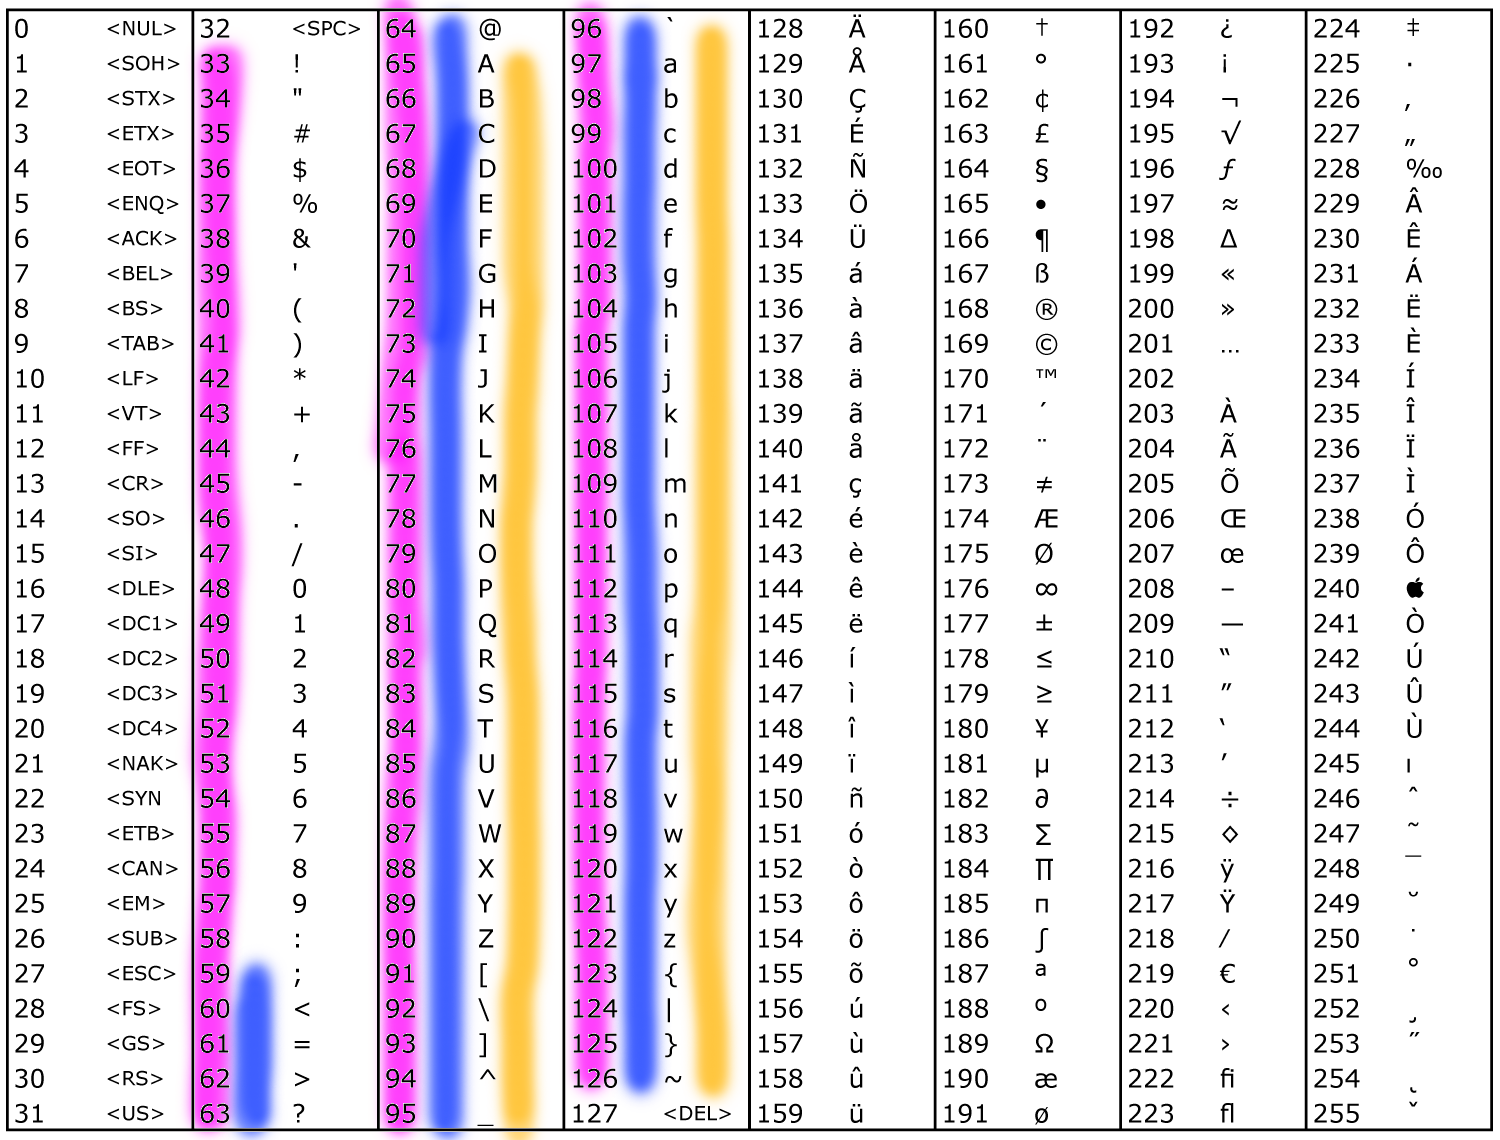
\includegraphics[height=0.7\textheight]{images/ascii_table}
    \end{center}  
\end{frame}

% FASTQ data format
\begin{frame}[fragile]
  \frametitle{FASTQ encoding\footnote{\tiny{\href{http://dx.doi.org/10.1093/nar/gkp1137}{Cock \textit{et al}. (2009) \textit{Bioinformatics} \textbf{38}:1767-1771 doi:10.1093/nar/gkp1137}}}}
  Versions vary by sequencer and period. Most now settled on Sanger format. \\
  Quality scores ($Q_{phred}$) offset to lie in the given range:
  \begin{enumerate}
    \item \textbf{Sanger}: 33-126, used in SAM/BAM, and Illumina 1.8+
    \item \textbf{Illumina 1.0-1.2}: 59-126
    \item \textbf{Illumina 1.3-1.8}: 64-126
  \end{enumerate}
  $Q_{phred} = -10 \log_{10}e$, where $e$ is the estimated probability that a base call is incorrect.
\end{frame}

% Variation in quality: good reads
\begin{frame}[fragile]
  \frametitle{Quality Control}
  The quality of basecalls varies along reads.\\
  \begin{center}
    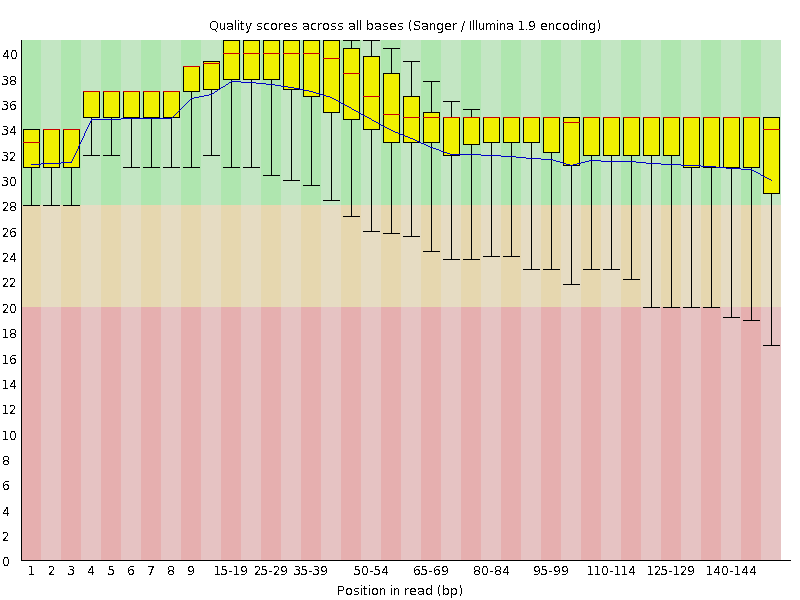
\includegraphics[height=0.6\textheight]{images/per_base_quality}
  \end{center}  
  (real data from our \textit{E.coli} sequencing: good quality)
\end{frame}

% Variation in quality: bad reads
\begin{frame}[fragile]
  \frametitle{Quality Control}
  Some datasets are better than others.\\
  \begin{center}
    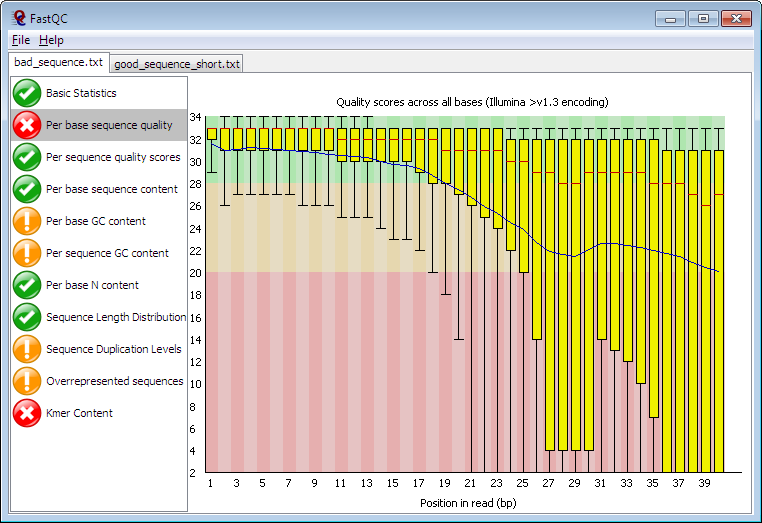
\includegraphics[height=0.5\textheight]{images/fastqc}
  \end{center}  
  Reads can be trimmed, or discarded.\\
  Including poor reads compromises assembly.
\end{frame}


% SUBSECTION: SAM/BAM/CRAM
% A very brief summary of the SAM/BAM/CRAM formats
\subsection{SAM/BAM/CRAM}

% SAM data format
\begin{frame}[fragile]
  \frametitle{SAM\footnote{\tiny{\href{http://samtools.github.io/hts-specs/SAMv1.pdf}{https://github.com/samtools/hts-specs}}}}
  \begin{center}
    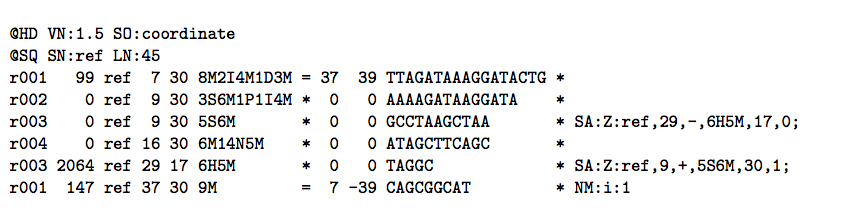
\includegraphics[width=0.8\textwidth]{images/sam_format}
  \end{center}  
  Intended to represent read alignments, also used for raw reads. \\
  Tab-delimited plain text. Headers (\textit{optional}) start with ``@'' \\
  \begin{center}
    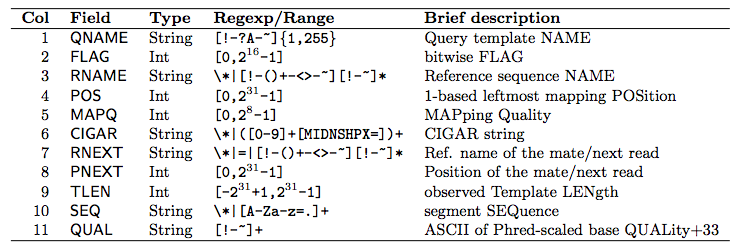
\includegraphics[width=0.8\textwidth]{images/sam_columns}
  \end{center}  
\end{frame}

% BAM data format
\begin{frame}[fragile]
  \frametitle{BAM\footnote{\tiny{\href{http://samtools.github.io/hts-specs/SAMv1.pdf}{https://github.com/samtools/hts-specs}}}/CRAM\footnote{\tiny{\href{http://www.ebi.ac.uk/ena/software/cram-toolkit}{http://www.ebi.ac.uk/ena/software/cram-toolkit}}}}
  BAM is a compressed version of SAM.\\
  \begin{itemize}
    \item BGZF compression.
    \item Random access within compressed file, through indexing.
  \end{itemize}
  CRAM format may come to dominate, especially in archives, as datasets get larger:
  \begin{itemize}
    \item Reference-based compression.\footnote{\tiny{\href{http://dx.doi.org/10.1101/gr.114819.110}{Fritz \textit{et al}. (2011) \textit{Genome Res.} \textbf{21}:734-740 doi:10.1101/gr.114819.110}}}
    \item Highly suited to compression and archiving of \textit{very} large amounts of sequence data.\footnote{\tiny{\href{http://dx.doi.org/10.1186/2047-217X-1-2}{Cochrane \textit{et al}. (2012) \textit{GigaScience} \textbf{1}:2 doi:10.1186/2047-217X-1-2}}}
  \end{itemize}  
\end{frame}



%%%
% SECTION: Sequence Assembly
\section{Assembly}
%% assembly_methods.tex
%% Author: Leighton Pritchard
%% Copyright: James Hutton Institute
%% These slides give a short, high-level account of the two dominant 
%% approaches to sequence assembly


% The two main approaches to sequence assembly
\begin{frame}
  \frametitle{Sequence Assembly}
  Two main approaches to read assembly:
  \begin{itemize}
    \item \textbf{Overlap-Layout-Consensus}: Typically used with smaller sets of longer reads (e.g. 454, PacBio, Ion, Nanopore)
    \item \textbf{de Bruijn assembly}: Typically used with many, shorter reads (e.g. Illumina), but also useful for longer reads
  \end{itemize}
  See e.g. Leland Taylor's thesis (\href{http://gcat.davidson.edu/phast/docs/Thesis_PHAST_LelandTaylor.pdf}{http://gcat.davidson.edu/phast/docs/Thesis\_PHAST\_LelandTaylor.pdf}), and PHAST (\href{http://gcat.davidson.edu/phast/index.html}{http://gcat.davidson.edu/phast/index.html}).
\end{frame}

% SUBSECTION: OLC
% A short account of Overlap-Layout-Consensus
\subsection{Overlap-Layout-Consensus}

% Graphical example of OLC
\begin{frame}
  \frametitle{Overlap-Layout-Consensus}
  \begin{center}
    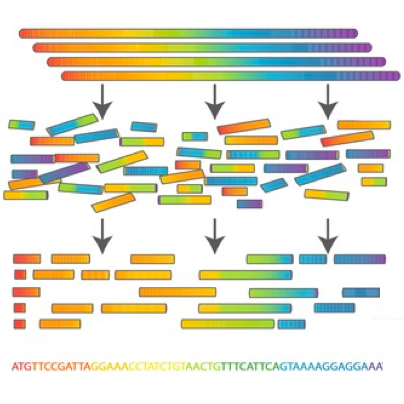
\includegraphics[height=0.8\textheight]{images/overlap-layout-consensus}
  \end{center}  
\end{frame}

% What tools use OLC, for which technologies
\begin{frame}
  \frametitle{Overlap-Layout-Consensus}
  The oldest approach, typically used with smaller sets of fewer reads. \\[0.5cm]
  Can be time consuming (all-vs-all comparisons), but offset with graph-based OLC algorithms (e.g. SGA).\\[0.5cm]
  \begin{itemize}
    \item Celera Assembler\footnote{\tiny{\href{http://wgs-assembler.sourceforge.net/}{http://wgs-assembler.sourceforge.net/}}}
    \item Newbler (the Roche/454 GS assembler)\footnote{\tiny{\href{http://www.454.com/products/analysis-software/}{http://www.454.com/products/analysis-software/}}}
    \item String Graph Assembler\footnote{\tiny{\href{http://dx.doi.org/10.1101/gr.126953.111}{Simpson and Durbin (2012) \textit{Genome Res.} \textbf{22}:549-556 doi:10.1101/gr.126953.111}}}
  \end{itemize}
\end{frame}

% SUBSECTION: de Bruijn graphs
% A short account of de Bruijn graph assembly
\subsection{de Bruijn graph assembly}

% Graphical examples of de Bruijn graphs
\begin{frame}
  \frametitle{de Bruijn graph assembly}
  $k$-mer based graph (choice of $k$ important):
  \begin{center}
    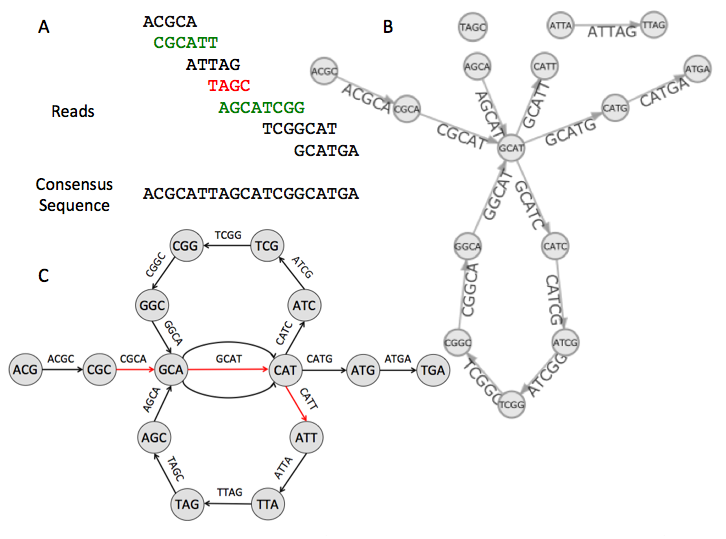
\includegraphics[width=0.8\textwidth]{images/deBruijn3}
  \end{center}  
\end{frame}

\begin{frame}
  \frametitle{de Bruijn graph assembly}
  $k$-mer based graph\footnote{\tiny{\href{http://dx.doi.org/10.1101/gr.079053.108}{Chaisson \textit{et al}. (2009) \textit{Genome Res.} \textbf{19}:336-346 doi:10.1101/gr.079053.108}}}
  \begin{center}
    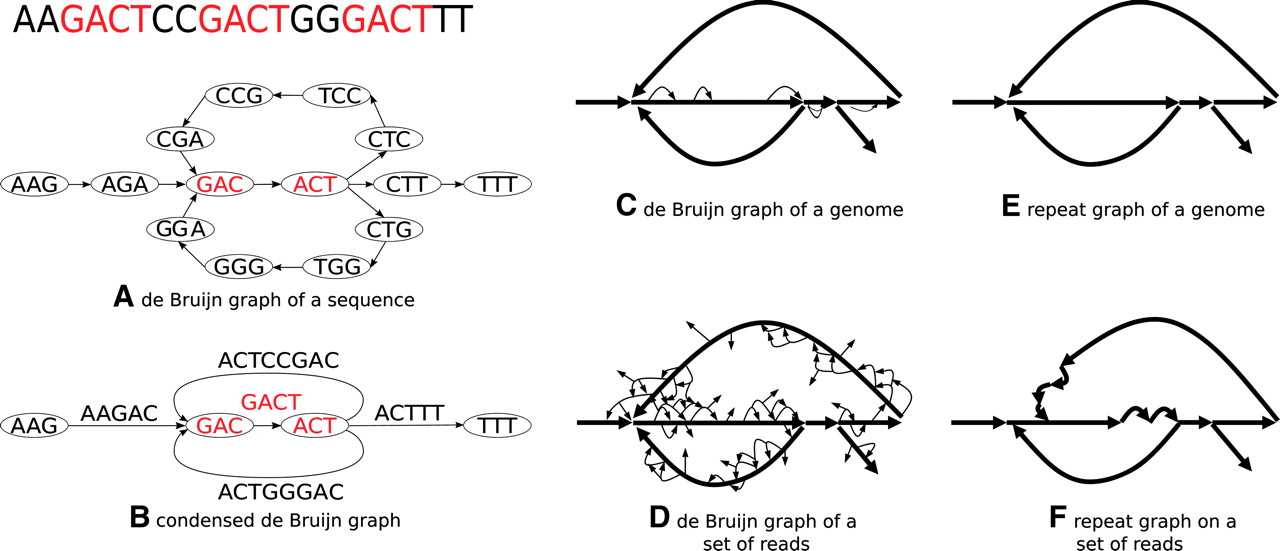
\includegraphics[width=1\textwidth]{images/de_bruijn_repeats}
  \end{center}  
\end{frame}

% What tools use OLC, for which technologies
\begin{frame}
  \frametitle{de Bruijn graph assembly}
  Fast, as it never computes overlaps.\\[0.5cm]
  Sensitive to sequencing errors, and repeats (graph bulges and whirls).\\[0.5cm]
  Notable tools:
  \begin{itemize}
    \item Velvet\footnote{\tiny{\href{http://dx.doi.org/10.1101/gr.074492.107}{Zerbino and Birney (2008) \textit{Genome Res.} \textbf{18}:821-829 doi:10.1101/gr.074492.107}}}
    \item CLC Assembly Cell\footnote{\tiny{\href{http://www.clcbio.com/products/clc-assembly-cell/}{http://www.clcbio.com/products/clc-assembly-cell/}}}
    \item Cortex\footnote{\tiny{\href{http://dx.doi.org/10.1038/ng.1028}{Iqbal \textit{et al}. (2012) \textit{Nat. Genet.} \textbf{44}:226-232 doi:10.1038/ng.1028}}}
  \end{itemize}
\end{frame}

% Graphical example of what else de Bruijn graphs can tell us
\begin{frame}
  \frametitle{``Coloured'' de Bruijn graph assemblies}
  Cortex\footnote{\tiny{\href{http://dx.doi.org/10.1038/ng.1028}{Iqbal \textit{et al}. (2012) \textit{Nat. Genet.} \textbf{44}:226-232 doi:10.1038/ng.1028}}} allows for on-the-fly identification of complex variation, and genotyping, by tracking ``coloured'' edges in the graph.
  \begin{center}
    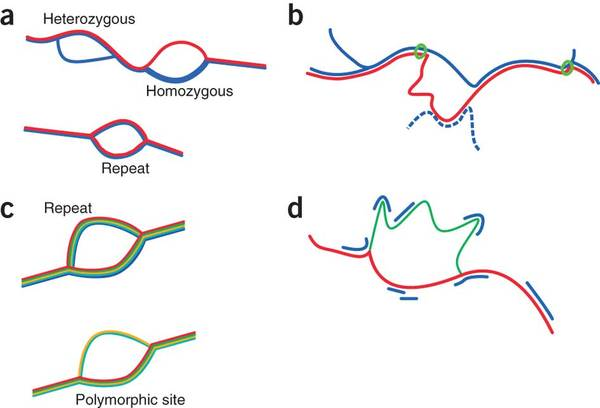
\includegraphics[width=0.8\textwidth]{images/cortex_uses}
  \end{center}  
\end{frame}




%%%
% SECTION: Read Mapping
\section{Read Mapping}
%% mapping.tex
%% Author: Leighton Pritchard
%% Copyright: James Hutton Institute
%% These slides give a short, high-level account of read mapping in 
%% sequence assembly

% SUBSECTION: Short-Read Sequence Alignment
% A short account of Read Mapping
\subsection{Short-Read Sequence Alignment}

% Graphical example of OLC
\begin{frame}
  \frametitle{Why map reads?\footnote{\tiny{\href{http://dx.doi.org/10.1038/nbt0509-455}{Trapnell \textit{et al}. (2009) \textit{Nat. Biotech.} \textbf{27}:455-457 doi:10.1038/nbt0509-455}}}}
  ``Resequencing'' an organism (really: a close relative, looking for SNPs/indels)\\
  To see where reads map on an assembled genome\\
  \begin{itemize}
    \item Is coverage even? (can indicate repeats)
    \item Are there SNPs/indels? (heterogeneous population)
    \item Assembly problems?
  \end{itemize}  
\end{frame}

% An overview of short-read sequence alignment
\begin{frame}
  \frametitle{Short-Read Sequence Alignment\footnote{\tiny{\href{http://dx.doi.org/10.1038/nbt0509-455}{Trapnell \textit{et al}. (2009) \textit{Nat. Biotech.} \textbf{27}:455-457 doi:10.1038/nbt0509-455}}}}
  An embarrassment of tools (over 60 listed on \href{http://en.wikipedia.org/wiki/List_of_sequence_alignment_software}{Wikipedia})\\
  Main approaches:
  \begin{itemize}
    \item \textbf{Alignment}: Smith-Waterman mathematically guaranteed to be the best alignment available (e.g. BFAST, MOSAIK);  approximation to S-W (e.g. BLAST); ungapped or gapped alignment (e.g. MAQ, FAST, mrFAST, SOAP). Can be slow.
    \item \textbf{Burrows-Wheeler Transform}: Makes permanent reusable index of the genome (e.g. Bowtie, BWA), can be extended to consider sequence probability (e.g. BWA-PSSM). Can be very fast.
  \end{itemize}
  Other tools may employ different algorithms, some designed to be parallelised on GPUs/FPGAs (e.g. NextGenMap, XpressAlign)
\end{frame}

% Graphical example of OLC
\begin{frame}
  \frametitle{Visualising Read Mapping}
  Several tools are available, e.g. Tablet\footnote{\tiny{\href{http://dx.doi.org/10.1093/bib/bbs012}{Milne \textit{et al}. (2013) \textit{Brief. Bioinf.} \textbf{14}:193-202 doi:10.1093/bib/bbs012}}}
  \begin{center}
    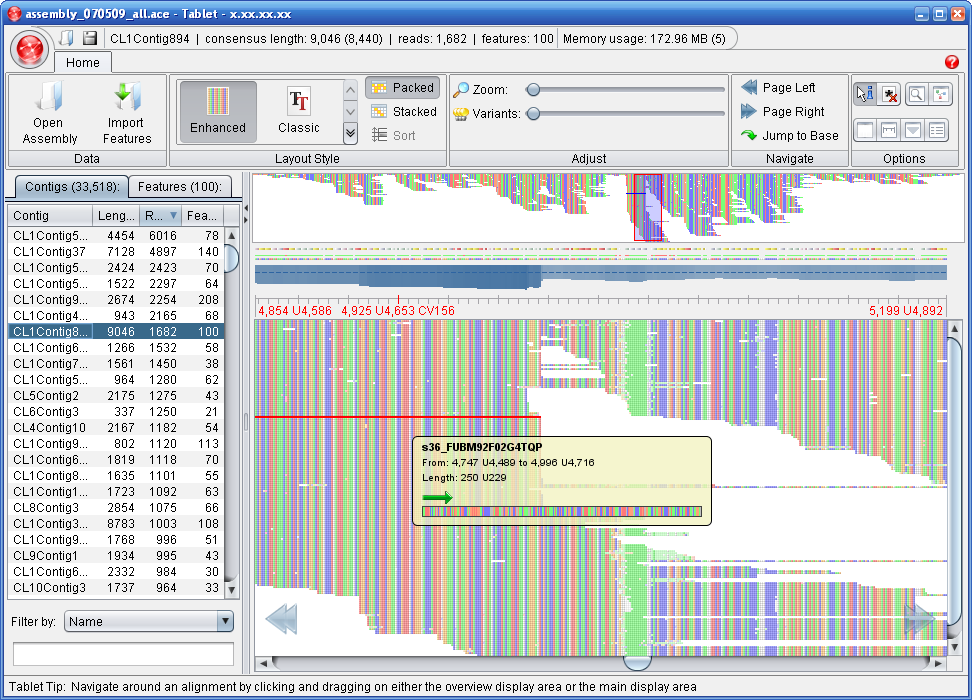
\includegraphics[height=0.65\textheight]{images/tablet1}
  \end{center}  
\end{frame}


%%%
% SECTION: Sequence Assembly
\section{The Assembly}
%% the_assembly.tex
%% Author: Leighton Pritchard
%% Copyright: James Hutton Institute
%% These slides give a short account of what you can 
%% expect back from sequence assembly

% SUBSECTION: What you get back
% What you get back from assembly
\subsection{What you get back}

% What you get back in an ideal world
\begin{frame}
  \frametitle{In an ideal world}
  Ideally, you would have one sequence per chromosome/plasmid.\\
  (and no errors): a \textbf{closed/complete} genome.
  \begin{center}
    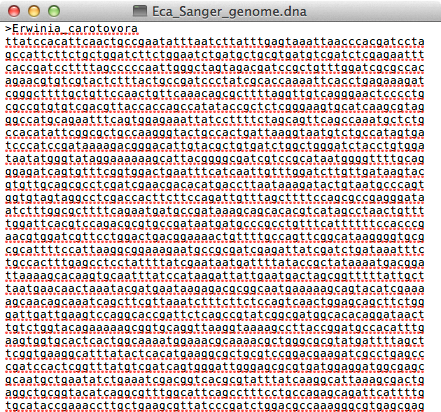
\includegraphics[width=0.5\textwidth]{images/pba_sequence}
    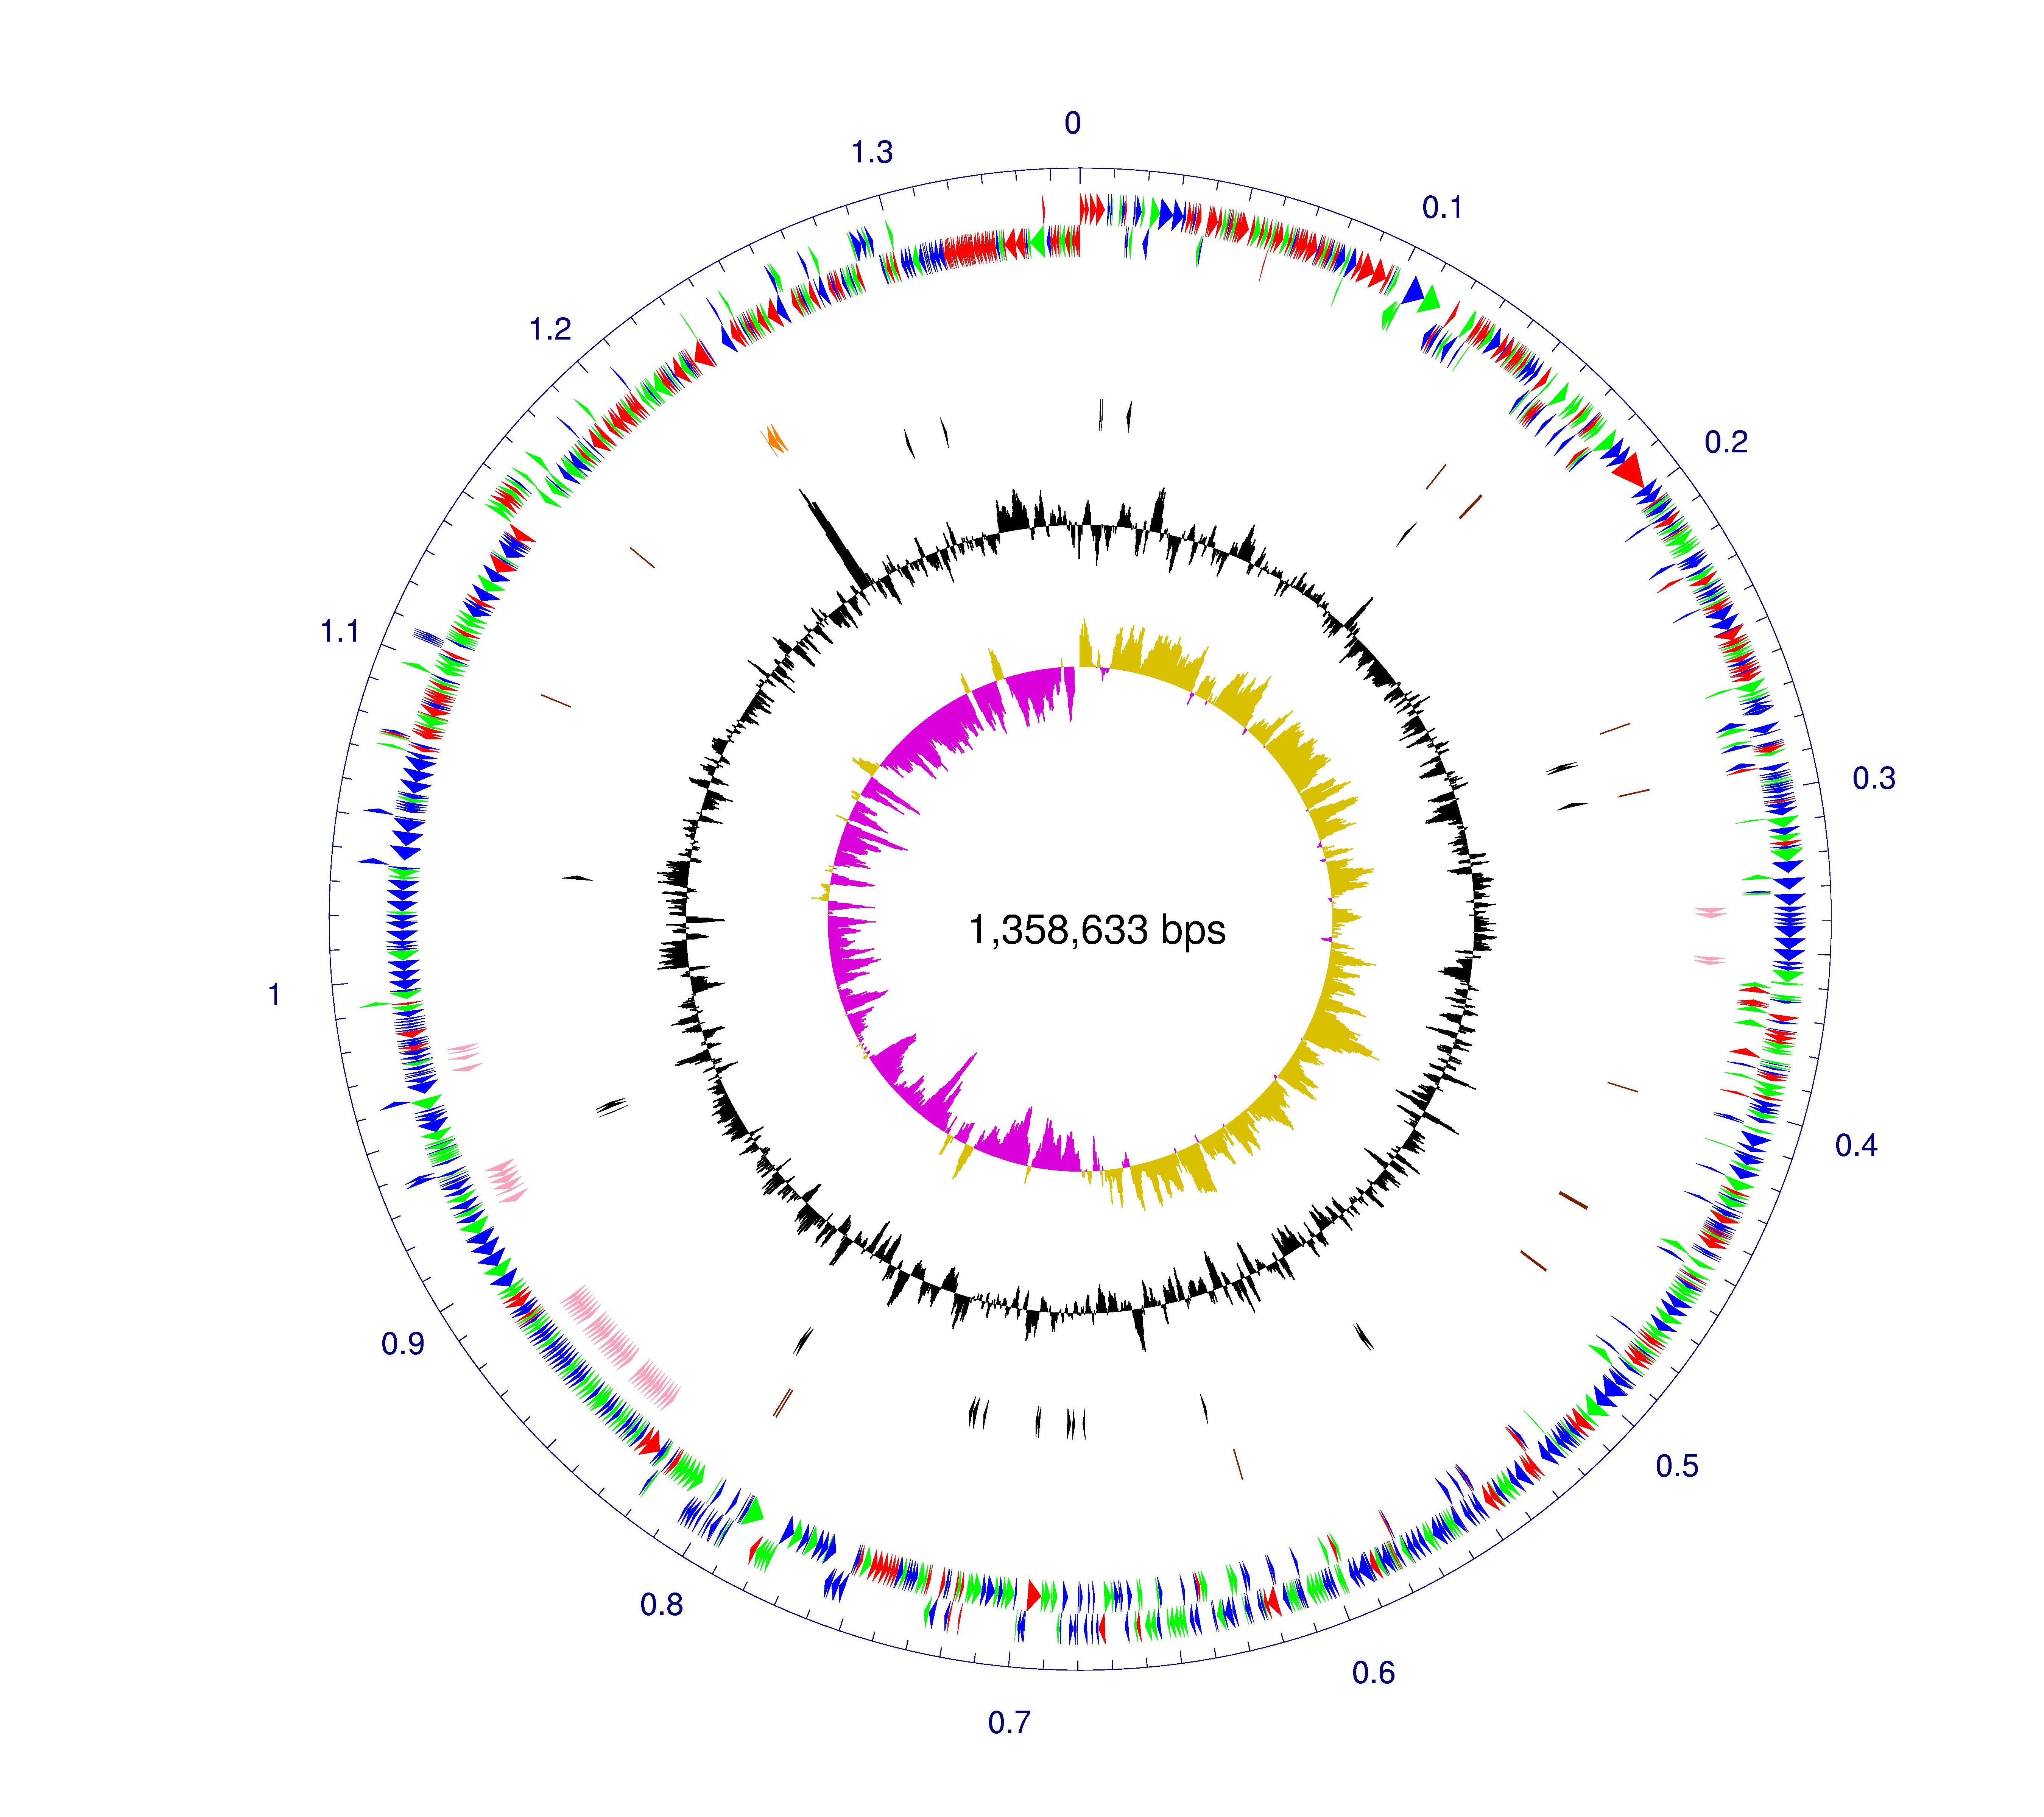
\includegraphics[width=0.5\textwidth]{images/complete_genome_circle}
  \end{center}    
  PacBio, Sanger, manual closing, Nanopore(?)
\end{frame}

% What you get back in an ideal world
\begin{frame}
  \frametitle{More realistically$\ldots$}
  Typically, a number of assembled fragments (contigs or scaffold) are returned in FASTA format: a \textbf{draft}, \textit{disordered} genome.\\
  Around 250 contigs for a 5Mbp genome is usual with Illumina\\
  \begin{center}
    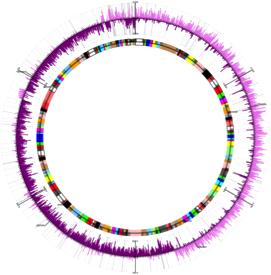
\includegraphics[width=0.5\textwidth]{images/circle_1}
    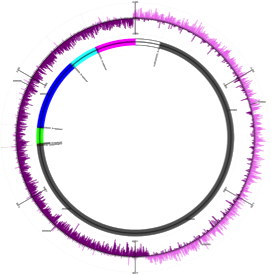
\includegraphics[width=0.5\textwidth]{images/circle_3}
  \end{center}    
\end{frame}

% Ordering fragments
\begin{frame}
  \frametitle{Ordering contigs}
  Contigs can be ordered correctly into \textit{scaffolds} if paired-end reads span gaps (typically done during assembly).\\
  Gaps are usually filled with \texttt{N}s (length estimated)
  \begin{center}
    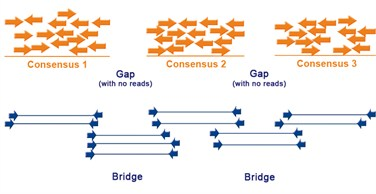
\includegraphics[width=1\textwidth]{images/contig_order_pe}
  \end{center}    
\end{frame}

% Ordering fragments
\begin{frame}
  \frametitle{Ordering contigs}
  Contigs and scaffolds can also be reordered by alignment to a reference genome.\\
  \begin{itemize}
    \item Mauve/progressiveMauve\footnote{\tiny{\href{http://dx.doi.org/10.1101/gr.2289704}{Darling \textit{et al}. (2004) \textit{Genome Res.} \textbf{14}:1394-1403 doi:10.1101/gr.2289704}}}
    \item MUMmer\footnote{\tiny{\href{http://dx.doi.org/10.1186/gb-2004-5-2-r12}{Kurtz \textit{et al}. (2004) \textit{Genome Biol.} \textbf{5}:R12 doi:10.1186/gb-2004-5-2-r12}}}
  \end{itemize}
  \begin{center}
    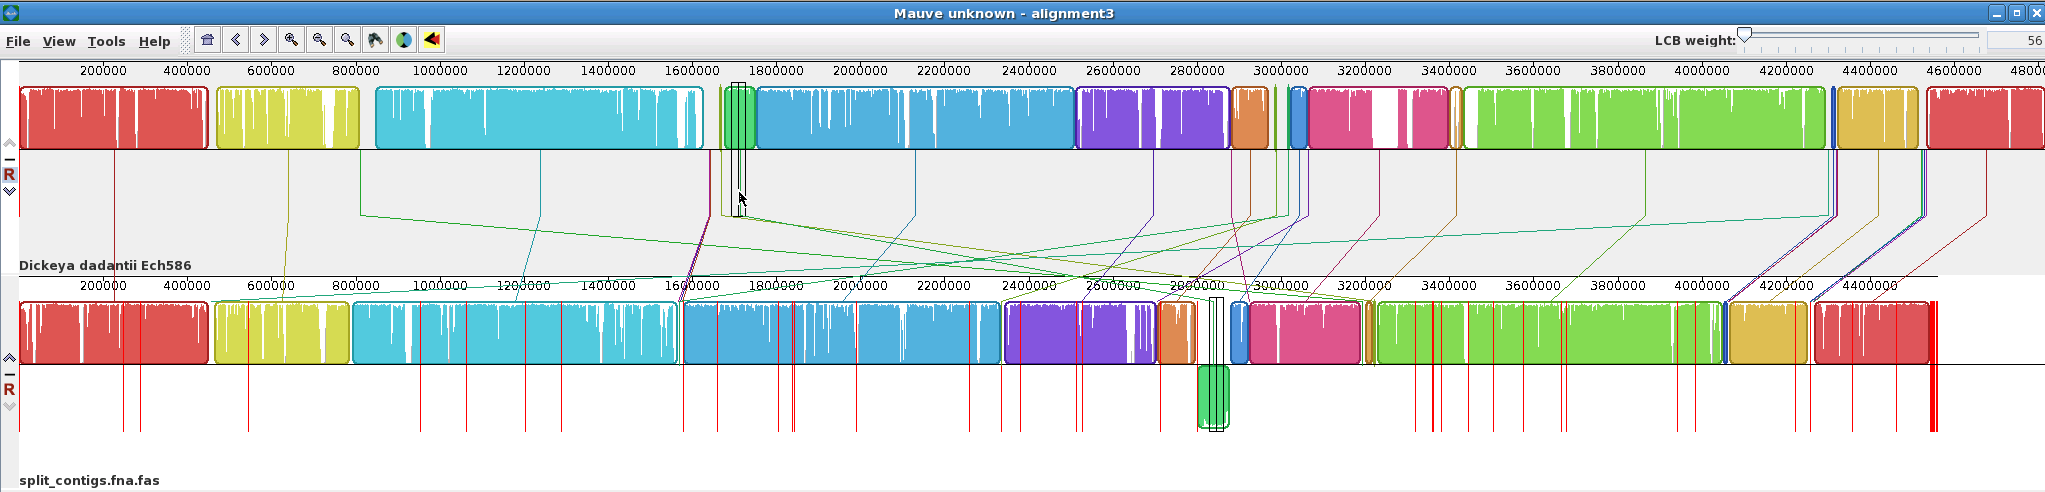
\includegraphics[width=1\textwidth]{images/mauve_output}
  \end{center}    
\end{frame}



%%%
% ACKNOWLEDGEMENTS
%\section{Acknowledgements}
%\input{sections/acknowledgements}


%%%
% LICENCE FOR REUSE
%% licence.tex
%% Author: Leighton Pritchard
%% Copyright: James Hutton Institute
%% These slides describe the licence for reuse of these slides and
%% materials

%
\begin{frame}
  \frametitle{Licence: CC-BY-SA}
  By: Leighton Pritchard \\[0.5cm]
  This presentation is licensed under the Creative Commons Attribution ShareAlike license \\
  \href{https://creativecommons.org/licenses/by-sa/4.0/}{https://creativecommons.org/licenses/by-sa/4.0/}
\end{frame}

% etc
\end{document}